\documentclass[12pt]{article}

\usepackage{scicite,times,graphicx,float,hyperref}
\usepackage[skip=0pt]{caption}
\usepackage[utf8]{inputenc}

\topmargin -1.0cm
\oddsidemargin 0.0cm
\textwidth 16cm 
\textheight 23cm
\footskip 1.0cm

\newenvironment{sciabstract}{%
\begin{quote} \bf}
{\end{quote}}

\newcounter{lastnote}
\newenvironment{scilastnote}{%
  \setcounter{lastnote}{\value{enumiv}}%
  \addtocounter{lastnote}{+1}%
  \begin{list}%
  {\arabic{lastnote}.}
  {\setlength{\leftmargin}{.22in}}
  {\setlength{\labelsep}{.5em}}
}
{\end{list}}

\title{Lab Work 3} 

\author
{André Pedrosa [85098], Filipe Pires [85122], João Alegria [85048]\\
\\
Algorithmic Information Theory\\
\normalsize{Department of Electronics, Telecommunications and Informatics}\\
\normalsize{University of Aveiro}\\
} 

\date{\today{}}

%%%%%%%%%%%%%%%%% END OF PREAMBLE %%%%%%%%%%%%%%%%

\begin{document} 

\baselineskip18pt

\maketitle 

\section{Introduction}
This report aims to describe the work developed for the third and final assignment
of the course of 'Algorithmic Information Theory', explaining all scripts
developed by us and presenting the results we considered most relevant Dataset
regarding the quality of the solutions. 

The programs implemented in Shell have the purpose of ...................Dataset
Dataset
Along with the description of the solutions, we also discuss .................
All code developed is publicly accessible in our GitHub repository:Dataset
\url{https://github.com/joao-alegria/TAI} .Dataset
\newpage

\section{Image Classification}
The challenge we are tackling in this paper is the one presented in \cite{trab3}, which is basically a image classification problem with a special approach. Instead of doing the process chosen by most people in charge of solving similar problems, consisting in using some from of feature extraction or some kind of feature learning commonly achieved through some type of machine learning algorithm, the launched challenge aims to reach a similar goal taking only in consideration the notion of algorithmic information.

Algorithmic information, also known as algorithmic entropy or Kolmogorov complexity, is the measure of information in a given data portion based on the theoretical algorithm that would be necessary to create that same data portion. Being a quite abstract definition, an example can clarify the concept: taking in consideration the string A="0101010101" and string B="0010100110", it is much simpler to define string A than string B, since for A we can simple say that it is the string "01" repeated 5 times, where for string B it's harder and we probably need to say the entire string to describe it. This means that in reality string A as less information than string B. To achieve the algorithmic information of each one, the thought process is the same but now the string descriptions are made with algorithms, where the string can be defined be the following algorithms:

\vspace{0.2in}
\begin{minipage}{0.45\textwidth}
  \begin{verbatim}
    def stringA():
      for i in range(5):
        print("01", end="")
  \end{verbatim}
\end{minipage}
\begin{minipage}{0.45\textwidth}
  \begin{verbatim}
    def stringB():
      for letter in "0010100110":
        print(letter, end="")
  \end{verbatim}
\end{minipage}
\vspace{0.2in}

Which by a quick iteration analysis its obvious that \texttt{stringA()} is less complex than \texttt{stringB()}, needing only 5 iterations compared with 10 iterations, respectively, confirming that string B has more information than string A. This can be directly correlated with data compression, since compressors take advantage of the data repetition as dispensable data, and thereby compress the information by removing repetition but storing an indicator of that repetition.

With this concepts defined it's more clear how the image classification will be done. Using the Normalized Information Distance(NID) defined by:

\begin{equation}
  NID(x,y) = \frac{max\{K(x|y),K(y|x)\}}{max\{K(x),K(y)\}}
\end{equation}

Where \textit{K(x)} defines the Kolmogorov complexity of the string x and \textit{K(x|y)} defines the Kolmogorov complexity of the string x given string y. Unfortunately, because the Kolmogorov complexity is non-computable this formula is only theoretical since there is no algorithm that can compute any string complexity every time. For that reason compressors are used to achieve approximations of the formula result. The studied approximations are Normalized Compression Distance(NCD) and Normalized Conditional Compression Distance(NCCD) that will be further detailed in the following subsections.

\subsection{NCD Approximation}
This approximation, which follows the Formula \ref{ncd} is frequently used to replace the NID. By using known general purpose compressors, such as gzip, lzma, tar, ..., the Kolmogorov complexity can be estimated by the number of bits the resulting compressed file has. 

\begin{equation}\label{ncd}
  NCD(x,y) = \frac{C(x,y)-min\{C(x), C(y)\}}{max\{C(x),C(y)\}}
\end{equation}

In Formula \ref{ncd}, \textit{C(x)} represents the number of bits the compression of x contains and \textit{C(x,y)} represents the number of bits the compression of x and y concatenated. This concatenation can be performed by several ways, the most common is to simply perform an union on both, but can be as complex as interlacing the two data sources. Following the formula, results close to 0 indicate similarity and close to 1 dissimilarity. The only restriction to this approach is that the compressor used must follow the condition $C(x,x) \simeq C(x)$, without that the results of NCD may not be reliable nor true. 

\subsection{NCCD Approximation}
This approach is yet another approximation to the NID formula, this time using conditional compressors to achieve their estimation. Conditional compressors are normally implemented with finite-context models and take in consideration the previous occurring terms to compress the new term. This is a more direct approximation of the NID and, in general, generate better results than the NCD. Defined by:

\begin{equation}
  NCCD(x,y) = \frac{max\{C(x|y), C(y|x)\}}{max\{C(x), C(y)\}}
\end{equation}

Where \textit{C(x)} defines once again the number of bits the compression of the object x by a given conditional compressor and $C(x|y)$ represents the number of bits the compression of x needs given that y occurred previously ($C(y|x)$ has the same logic). Due to the consitional aspect of this approach, \textit{C(x)} can be a special case of $C(x|y)$ were y is equal to the empty string, causing that $C(x) = C(x|\epsilon)$.

\newpage
\section{Dataset}
Lorem ipsum ...

% \begin{figure}[H]
%   \centering
%   \begin{minipage}{\textwidth}
%     \centering
%     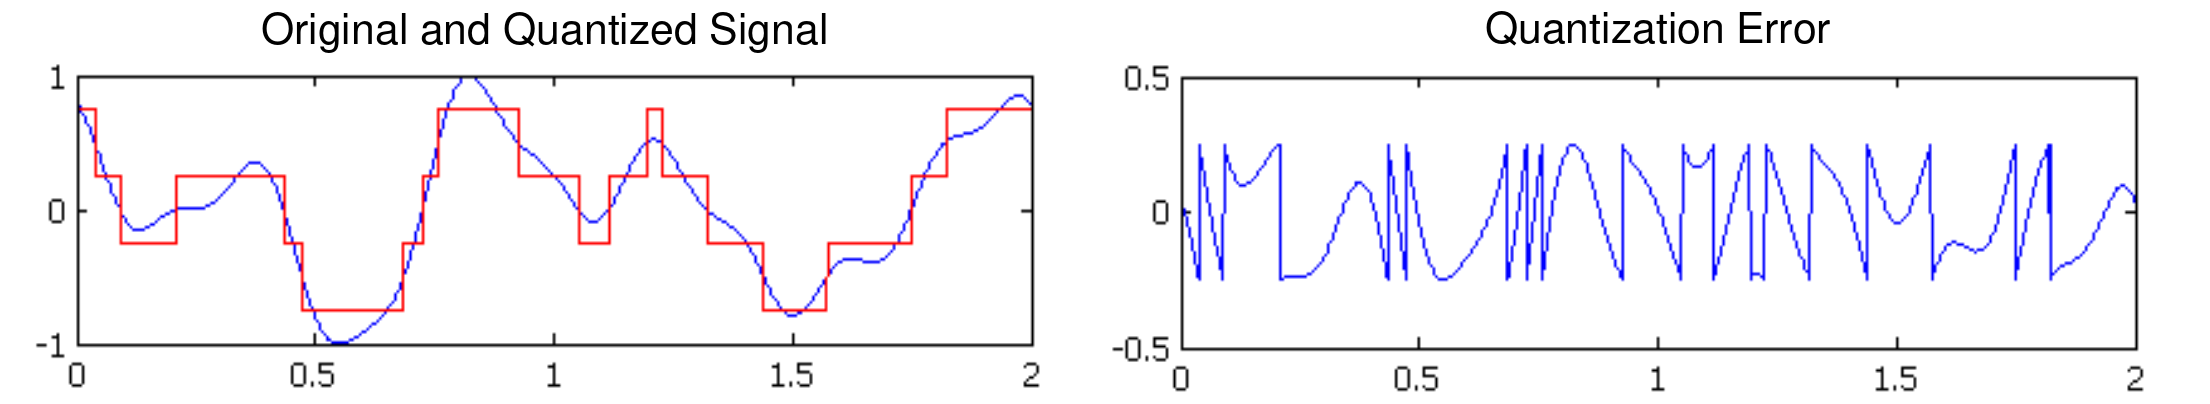
\includegraphics[width=\linewidth]{stanford_quantization_wide.png}
%   \end{minipage}%
%   \caption{Example of a quantized waveform.}
%   \label{fig:quantization}
% \end{figure}

\section{Experiment}
Lorem ipsum ...

\subsection{Tested Compressors}
.......

\section{Results \& Discussion}
Lorem ipsum ...


\section{Conclusions}

After completing the assignment, we drew a few conclusions regarding our 
solutions and ..................

Lorem ipsum ...

In terms of code organization and readability, we made sure our 
repository was as well structured as possible and our code properly commented
and documented.
The base folder contains a {\it README\/} file for basic instructions.
All code is in the {\it src\/} folder.

\newpage
\begin{thebibliography}{9}
  \bibliographystyle{Science}

  \bibitem{trab3}
    Armando J. Pinho,
    \textit{AIT: Lab Work no.3},
    University of Aveiro,
    2019/20.
  
\end{thebibliography}

\clearpage

\end{document}




















